% !TeX root = ../main.tex
% Add the above to each chapter to make compiling the PDF easier in some editors.

\begin{figure}[t!]
    \centering
    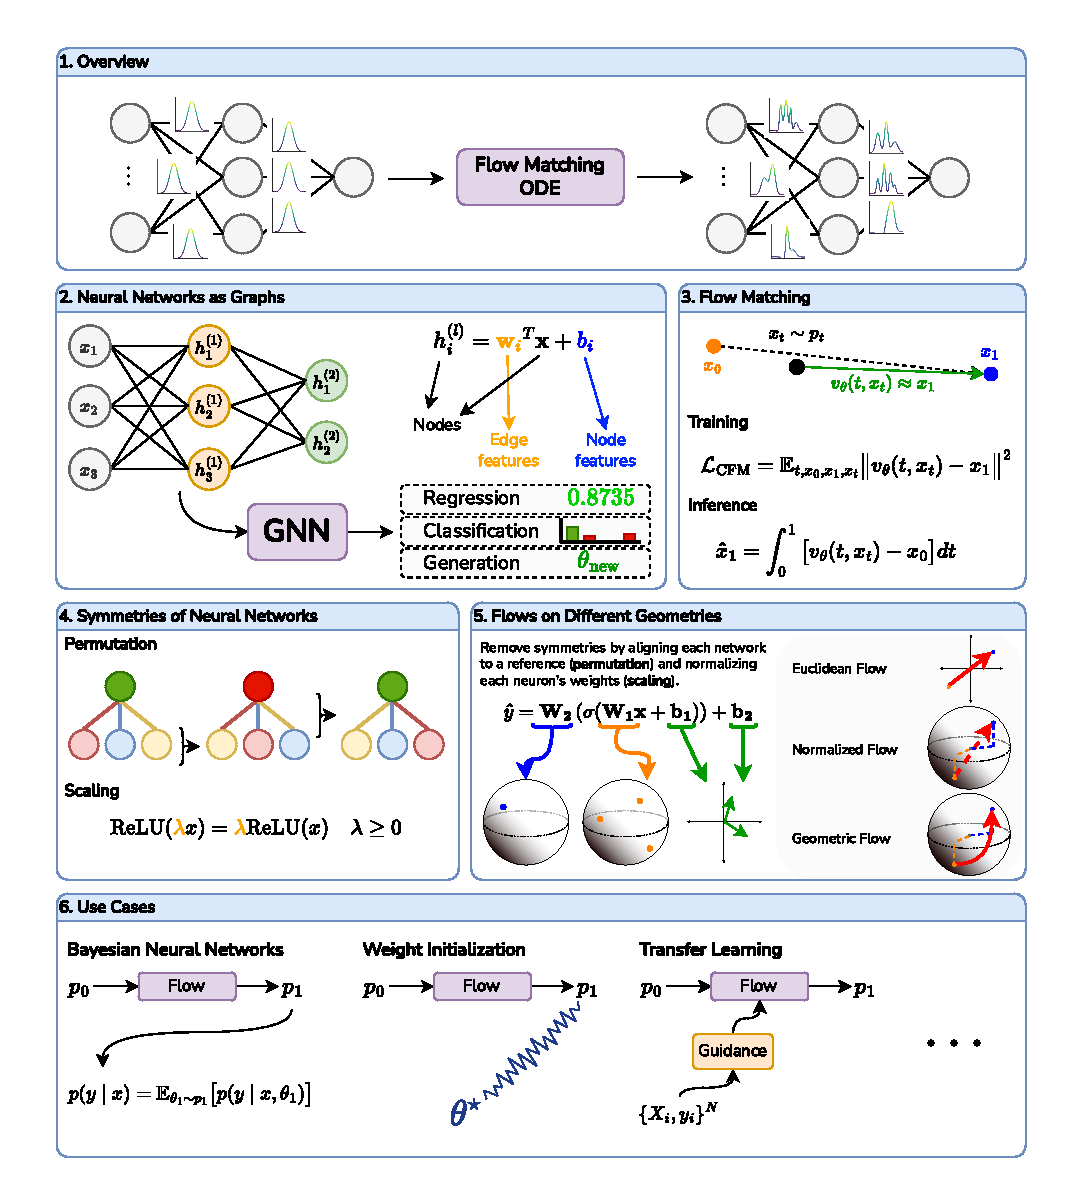
\includegraphics[width=\linewidth]{figures/weightflow.drawio.pdf}
    \caption{\label{fig:main}\textbf{Overview of our weight-space flow.} We aim to learn a flow in weight-space \textit{(1)}, processing neural networks with GNNs \textit{(2)}, using flow matching \textit{(3)} and taking into account the symmetries of neural network weights \textit{(4)}. We propose three different flows \textit{(5)} and potential use cases include Bayesian neural networks, learned weight initialization, or transfer learning \textit{(6)}.}
\end{figure}

\chapter{Introduction}\label{chapter:introduction}

Deep generative models such as diffusion and flow models that have led to significant developments in image generation \citep{esserScalingRectifiedFlow2024b} and biological applications such as protein structure prediction \citep{abramsonAccurateStructurePrediction2024} have also been applied to neural network weights \citep{peeblesLearningLearnGenerative2022,schurholtHyperRepresentationsLearningPopulations2024a}. However, the existing works do not take into account the geometry of neural networks arising from permutation and scaling symmetries, or only consider the permutation symmetries. However, modeling the symmetries of data often leads to improved performance and more data-efficient training \citep{brehmerDoesEquivarianceMatter2024}. We attempt to fill this gap by building flow models that learn a vector field to transport a prior over neural network to the posterior for a specific task through the flow matching framework \citep{lipmanFlowMatchingGuide2024}, processing neural network weights with permutation-invariant graph neural networks \citep{kofinasGraphNeuralNetworks2024,limGraphMetanetworksProcessing2023} and propose three candidate designs differing on how they handle the underlying geometry. Figure \ref{fig:main} gives an overview of our approach, and we summarize the main points in this Introduction. 

\section{Motivation}

\subsubsection*{Weight-Space Generative Models as Learned Optimizers}

A generative model of neural network weights is in essence a learned optimizer, and learned optimizers constitute an active research area in their own right \citep{hospedalesMetaLearningNeuralNetworks2022}. However, unlike typical learned optimizers that are often trained by unrolling the gradient-based optimization of neural networks \citep{finnModelAgnosticMetaLearningFast2017}, generative models are trained directly with data (trained neural network weights), using the outputs of neural network training. This implies weight-space generative models can be improved by utilizing public datasets of neural network checkpoints such as \citep{peeblesLearningLearnGenerative2022,schurholtModelZoosDataset2022}.

Inference with weight-space generative models is also fundamentally different than gradient-based optimization. Rather than predict the task gradients or output optimization steps, a generative model can output trained weights in ``one-shot.'' Furthermore, they open the way for applications of tools from the modern generative models literature to navigate the space of neural network weights. 

\subsubsection*{Weight-Space Generative Models as Probabilistic Models}

The fundamental units of modern generative models such as diffusion and flow models are probability distributions, that is they learn to transport one probability distribution such as a Normal distribution to another one such as the distribution of certain images. Weight-space generative models therefore also model a complex probability distribution over neural network weights. They can both efficiently sample from it, and evaluate the likelihood of arbitrary points under this distribution. 

Being able to both sample from and evaluate the likelihood function of a complex distribution puts generative models in a unique place among similar methods. The likelihood function of variational approximations of neural network posteriors can also be evaluated, but they model considerably simpler distributions, while Markov chain Monte Carlo methods can sample from more complex multi-modal distributions but do not allow likelihood computations. Nevertheless, this power of generative models comes with increased computational demands during training and the need for careful architecture design. 


\subsubsection*{Generative Models, Geometry, and Neural Network Weights}

Geometric generative models that model the geometry of their domain by invariance/equivariance constraints \citep{kleinEquivariantFlowMatching2023a}, parametrizing their data points on manifolds \citep{chenRiemannianFlowMatching2023}, or learning a manifold structure from data points alone \citep{kapusniakMetricFlowMatching2024} have been applied to a wide range problems from climate modeling \citep{bodnarAuroraFoundationModel2024} to protein design \citep{boseSE3StochasticFlowMatching2024}. By baking in the correct inductive biases from the start rather than expecting a model to learn them from scratch or through data augmentation, such geometric models make training more data-efficient. 

It is thus a logical first-step, especially for high-dimensional and multi-modal distributions such as neural network posteriors, to model the geometric structure of the data as accurately as possible. In particular for deep neural networks, their non-identifiability - there being multiple parametrizations of the same function, is a key reason behind this multi-modality, and it is hypothesized that the modes in a neural network posterior are actually linearly connected up to function-preserving permutations \citep{entezariRolePermutationInvariance2022}. Together, these considerations motivate that weight-space learning tasks can be considerably simplified through appropriate geometric modeling choices. 


\section{Overview}

\subsubsection{Symmetries of Neural Networks (Chapter \ref{section:geometry_of_nns})}

Neural network weights possess various symmetries, i.e. transformations of the network parameters that leave the function it is computing unchanged, and this topic has been an active research area since the early days of neural network research \citep{hecht-nielsenALGEBRAICSTRUCTUREFEEDFORWARD1990}. For example in an MLP, permuting the neurons in one layer together with the outgoing weights preserves the function, as does similarly permuting the channels in a convolutional neural network. Non-linear activation functions induce further scaling symmetries \citep{godfreySymmetriesDeepLearning2022}; e.g. for a constant $\lambda \geq 0$, $\text{ReLU}(\lambda x) = \lambda \text{ReLU}(x)$, which means scaling the input weights to a neuron and applying the inverse scaling to the outgoing weights again preserves neural network's function. In addition to these static symmetries, other forms of symmetries might arise from the structure of the data, or dynamically during periods of training \citep{zhaoFindingSymmetryNeural2024}. 

Accounting for these symmetries in a weight-space learning task by using architectures with the correct inductive biases, through data augmentation \citep{shamsianImprovedGeneralizationWeight2024}, or by removing the symmetries by mapping neural networks to canonical representations \citep{pittorinoDeepNetworksToroids2022} as we will do can reduce the effective dimensionality of the problem and make weight-space learning more efficient. 

\subsubsection{Neural Networks as Graphs (Chapter \ref{section:wsl})}

A neural network can naturally be modeled as a graph, and this has fueled a recent line of work building graph neural networks (GNNs) that take as input other neural networks \citep{kofinasGraphNeuralNetworks2024,limGraphMetanetworksProcessing2023,kalogeropoulosScaleEquivariantGraph2024}. The nodes often correspond to the neurons in an MLP or channels in a convolutional network and the edges to the weights. Used with the appropriate positional encodings, this graph formalism provides an effective way of handling the permutation symmetries of various kinds of neural networks including transformers and neural networks with residual connections, and has also been extended to account for scaling symmetries \citep{kalogeropoulosScaleEquivariantGraph2024}. Furthermore, since a GNN is not restricted to graphs with a certain structure, weight-space GNNs have the additional benefit that the same GNN can be used to process different neural networks, even those with different architectures altogether.

As part of our flows, we process neural networks using GNNs, more specifically the Relational Transformer architecture \citep{diaoRelationalAttentionGeneralizing2023,kofinasGraphNeuralNetworks2024} that incorporates an attention mechanism with edge updates. 

\subsubsection{Generative Modeling with Flow Matching (Chapter \ref{section:flow_models})}

Flow matching (FM) \citep{lipmanFlowMatchingGenerative2023,albergoStochasticInterpolantsUnifying2023,liuFlowStraightFast2022,tongImprovingGeneralizingFlowbased2023} generalizes diffusion models with a more flexible framework and a simple simulation-free regression objective. Given two sampleable marginal distributions $p_0$ and $p_1$, a coupling $(x_0, x_1)$ is sampled from a joint distribution, and $x_t$ from the intermediate distribution $p_t(x_t \mid x_0, x_1)$ conditioned on the endpoints with $t$ sampled within the interval $[0,1]$. A neural network (velocity model) is then trained to predict the conditional velocity $u_t(x_t \mid x_0, x_1)$, such as $x_1 - x_0$. Marginalizing this linear vector field over the joint coupling then results in a more complex vector field that transforms $p_0$ to $p_1$, which is estimated by solving a differential equation with the velocity given by the trained velocity model. This flow matching framework can also be extended to data with more general geometries such as Riemannian manifolds \citep{chenRiemannianFlowMatching2023}. 

We will train our models using flow matching, with a Gaussian prior and the posterior samples collected through the neural networks' optimization trajectories, experimenting with different couplings. Our slightly modified flow matching training setup is described in more detail in Section \ref{sec:fm_training}.

\subsubsection{Flows with Different Geometries (Chapter \ref{chapter:method})}

We propose three flow models that handle the underlying geometric structure in different ways, which enables us to evaluate the effect of geometric considerations more precisely. We consider ReLU MLPs, and first align all neural networks to the same reference network using the rebasin operation \citep{ainsworthGitReBasinMerging2023,penaReBasinImplicitSinkhorn2023} that permutes a network's weights to minimize the loss barrier between two networks.  To handle the scaling symmetries, we build on the canonicalization procedure of \citep{pittorinoDeepNetworksToroids2022}, where each neuron's incoming weights are normalized and its outgoing weights are inversely scaled to preserve the function being computed; the last layer is further normalized globally in classification networks. This gives the neural network a product geometry, with the bias vectors as Euclidean vectors, intermediate neurons' incoming weight vectors on the hypersphere, and the last layer (optionally) on the hypersphere as a whole. 

We then compare our three flows: first a Euclidean flow that ignores the scaling symmetries and models each weight vector in Euclidean space, then a Normalized flow with the weights embedded in the product geometry but with the velocity field defined in Euclidean space (i.e. inside the hyperspheres), and finally a Geometric flow with the velocity field defined on the product geometry as well using the Riemannian Flow Matching framework \citep{chenRiemannianFlowMatching2023}. 

\subsubsection{Overview of Results (Chapter \ref{chapter:results})}

We evaluate our flows on a variety of tasks after training them on samples obtained with gradient-based optimization methods and show that for small networks on relatively easier tasks, they can directly generate weights matching or sometimes exceeding the performance of weights optimized with gradient-based methods. On more complex tasks and larger models, while direct generation does not match the quality of optimized weights, Bayesian model averaging over a number of samples leads to comparable predictive performance. Then we show that a flow trained on weights from one task can be transferred to another task, either by using the sampled weigths as learned initializations, or by guiding the sampling process with task gradients. Our results finally demonstrate that in particular the Euclidean and Geometric flows can also generalize to different architectures for the same base task, and that there are still gains to be made by further scaling up our models. 

\section{Contributions}

Our main contributions are as follows:
\begin{itemize}
    \item We utilize flow matching in weight-space for the first time. Our Euclidean flow learns to transport weights in Euclidean space directly, then we model the neural networks on a product manifold by removing their scaling symmetries to build our Normalized flow, and finally in our Geometric flow we utilize the Riemannian Flow Matching framework to define a vector field over this product manifold. 
    \item We empirically validate our proposed methods by learning to approximate the posterior distributions of neural networks of various sizes on different tasks. We observe that they can generate samples competitive with weights optimized via gradient-based methods, and that can still be scaled up for better performance. 
    \item We show that our flows can also generalize to different architectures, such as by sampling more accurate weights for a larger mode. This indicates they do not learn to model just a single posterior distribution, but instead learn to model weights on the underlying task more generally. 
    \item Finally we apply guidance with task gradients during sampling as an instance of transfer learning and show that a flow built with weights trained on one dataset can be used to sample weights that are accurate on another dataset. 
\end{itemize}